%!TEX root = ../apese-rapport.tex
\section{Nos outils}
	Étant sur trois systèmes d'exploitations différents et ayant des affinités avec différents outils, nous avons utilisé des outils différents :
	\begin{itemize}
		\item Atom, un éditeur de texte libre pour macOS, GNU/Linux et Windows développé par GitHub.
		Il a la particularité de pouvoir se transformer en IDE.
		\item Eclipse, un IDE principalement utilisé dans la programmation Java. C'est même le plus utilisé chez les développeurs Java.
		\item Neovim, un éditeur de code accessible depuis le terminal. C'est une version améliorée de Vim qui était, lui, une amélioration de Vi (Vi IMproved).
		\item Visual Studio Code, un éditeur de code extensible développé par Microsoft pour macOS, GNU/Linux et Windows, et basé sur Atom.
		Il a la particularité d'être compatible, de base, avec TypeScript.
	\end{itemize}

\begin{figure}[ht]
	\centering
	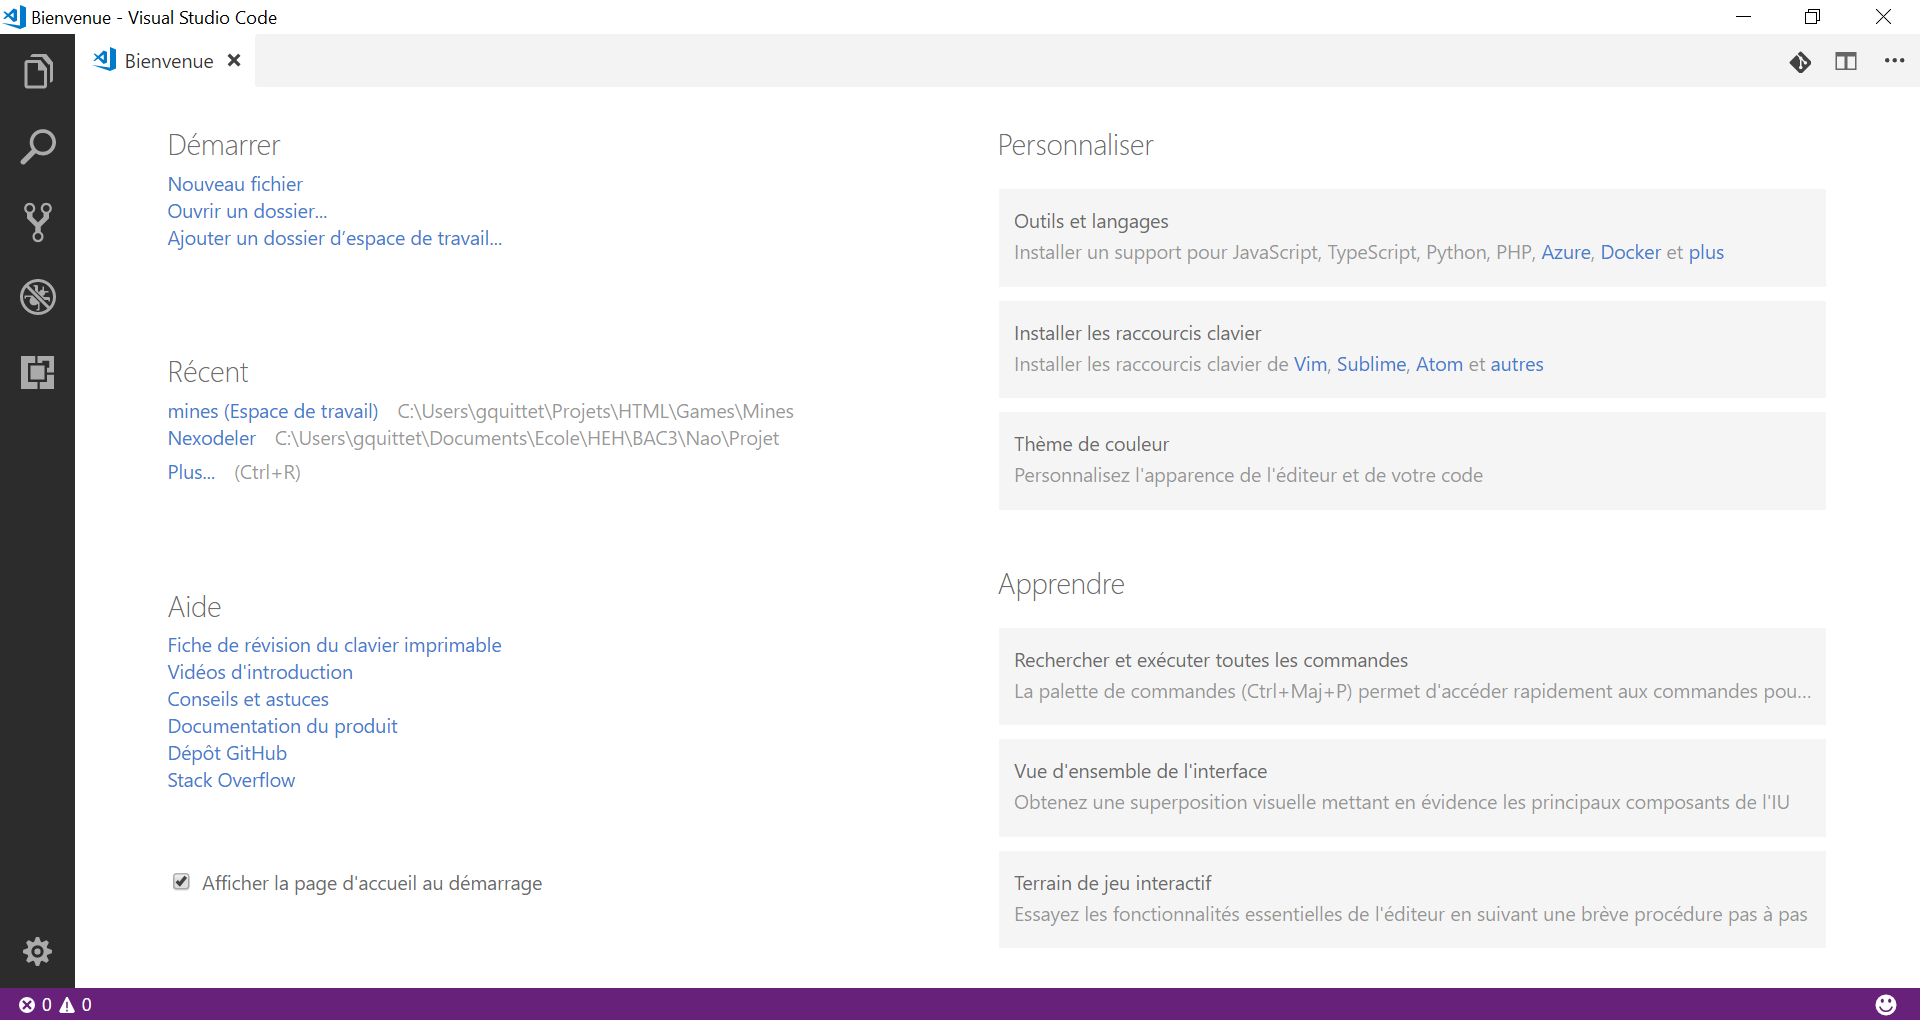
\includegraphics[width=\textwidth]{vs-code-interface.PNG}
	\caption{Interface de Visual Studio Code}
\end{figure}
